\section{Lecture 3}

\subsection{Exponential Map}

Recall that for two dimensions, we can parameterize angles like this:
\[ e^{i \phi} = \cos \phi + i \sin \phi \]
These form the set $S^1 = \{z \in \C \mid |z| = 1\}$
To do this, we need a few notions first.

Recall that the differential equation:
\begin{align*}
    \dot{x}(t) = ax(t) \\
    x(0) = x_0
\end{align*}
has the soution $x(t) = e^{at} x_0$. The same solution generalizes quite easily to a vector system,
with a matrix exponential instead of a scalar one.

Consider some matrix $R \in SO(3)$. Then, there are 6 orthogonality constraints:
\[ r_i \cdot r_j = \begin{bmatrix}
    0 & i \neq j \\
    1 & i = j
\end{bmatrix} \]
which means 3 independent degrees of freedom I can pick.

Now, consider the motion of a point $q$ on a rotating link. The motion is given by the differential equation:
\begin{align*}
    \dot{q}(t) = \omega \cross q(t) = \hat{\omega} q(t) \\
    q(0) = q_0
\end{align*}
where $\omega$ points in the direction of the axis we are rotating about.
We can solve this is the same way as before!
\[ q(t) = e^{\hat{\omega} t} q_0 \]
where of course, the matrix exponential is:
\[ e^{\hat{\omega} t} = I + \hat{omega}t + \frac{(\hat{omega} t)^2}{2!} + \dots \]

We can then consider the following map, supposing $\hat{\omega}$ has unit norm and now we are rotating by some angle $\theta$
instead of for some time $t$ (hence why we need normalization to rotate at unit speed).
\begin{definition}[Exponential Map]
    \[ \exp: so(3) \to SO(3), \hat{\omega} \theta \mapsto e^{\hat{\omega} \theta} \]
\end{definition}

i.e. we are claiming that $e^{\hat{\omega} \theta}$ is a rotation matrix. We will see this later.

It turns out we can write this infinite summation as a finite one, using Rodrigues' formula (again with unit norm assumption).
\[ e^{\hat{w} \omega} = I + \hat{\omega} \sin \theta + \hat{\omega}^2 (1 - \cos \theta) \]
The first part of the proof is pretty bashy. I have attached a screenshot to save my fingers.

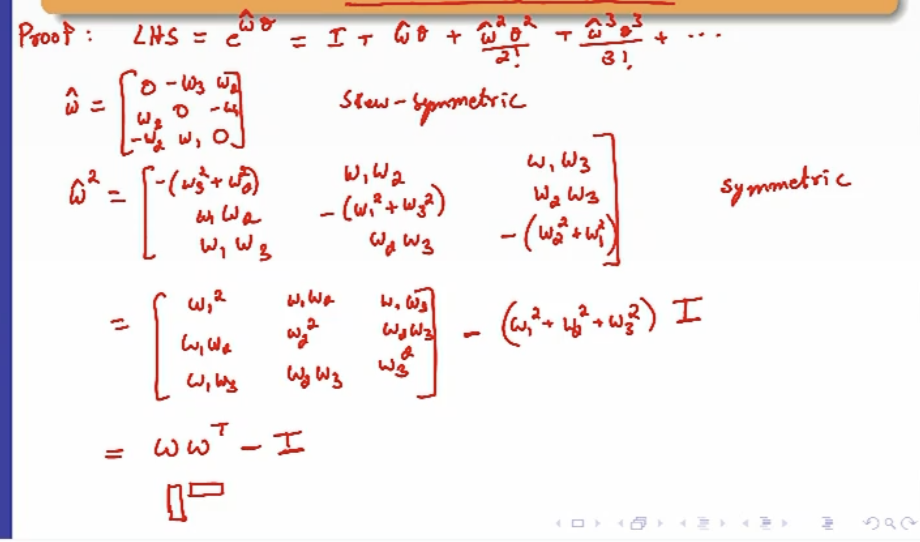
\includegraphics[width=400px]{rod-proof-1.png}

Continuing on, we have:
\begin{align*}
    \hat{\omega}^3 &= \hat{\omega}(\omega \omega^T - I) = \hat{\omega} \omega \omega^T - \hat{\omega} = - \hat{\omega} \\
    \hat{\omega}^4 &= \hat{\omega} (-\hat{\omega}) = - \hat{\omega}^2 \\
    \hat{\omega}^5 &= \hat{\omega} \\
    &\vdots 
\end{align*}

Then we have:
\[ e^{\hat{\omega} \theta} = I + \hat{\omega} \qty[\theta - \frac{\theta^3}{3!} + \dots] + \hat{\omega^2} \qty[\frac{\theta^2}{2!} - \frac{\theta^4}{4!} + \dots ] \]
which is exactly the claim (these are the power series of sin and cos).

Without the unit norm assumption, the full formula is:
\begin{theorem}[Rodrigues' Formula]
    For a vector $\omega$ and scalar $\theta$ we have:
    \[ e^{\hat{\omega} \theta} = I + \frac{\hat{\omega}}{\norm{\omega}} \sin \norm{\omega} \theta + \frac{\hat{\omega}^2}{\norm{\omega}^2}(1 - \cos \norm{\omega} \theta) \]
\end{theorem}

We will now show that this exponential map is a rotation.
\begin{proof}
    Let $R = e^{\hat{\omega} \theta}$. Then:
    \begin{align*}
        R^{-1} &= e^{-\hat{\omega} \theta} \\
        &= e^{\hat{\omega}^T \theta} \\
        &= \qty(e^{\hat{\omega} \theta})^T \\
        &= R^T
    \end{align*}

    Let us also see that the determinant is 1. We know from orthogonality of $R$ that it
    must have determinant either $-1$ or $1$. However,
    \[ \det \exp(0) = 1 \]
    and the determinant is continuous with respect to $\theta$, so it cannot jump to $-1$. Thus,
    the determinant must always be 1 and we have $e^{\hat{\omega} \theta} \in SO(3)$.
\end{proof}

Furthermore, the exponential map is onto.
\begin{proof}
    Given a rotation $R \in SO(3)$, there is some $\omega$ with unit norm and $\theta$ such that:
    $R = e^{\hat{\omega} \theta}$. Let
    \[ R = \begin{bmatrix}
        r_{11} & r_{12} & r_{13} \\
        r_{21} & r_{22} & r_{23} \\
        r_{31} & r_{32} & r_{33}
    \end{bmatrix} \]
    and $v_{\theta} = 1 - \cos \theta, c_{\theta} = \cos \theta, s_{\theta} = \sin \theta$
    By Rodrigues' formula (again I'm lazy):
    
    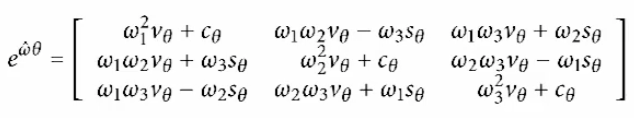
\includegraphics[width=400px]{hard-rod.png}

    Now we want to recover $\omega$ and $\theta$ to conclude the proof. Consider the trace of this matrix:
    \begin{align*}
        \tr(R) &= \omega_1^2 v_{\theta} + c_{\theta} + \omega_2^2 v_{\theta} + c_{\theta} + \omega_3^2 v_{\theta} + c_{\theta} \\
        &= 1 + 2 c_{\theta} \\
        &= \sum_{i = 1}^3 \lambda_i
    \end{align*}
    Now we have a few cases (which then we can figure out stuff by adding and subtracting equations).
    \begin{itemize}
        \item Case 1: $\tr(R) = 3$ or $R = I$, $\omega = 0 \implies \omega \theta = 0$.
        \item Case 2: $-1 < \tr(R) < 3$
        \[ \theta = \arccos \frac{\tr(R) - 1}{2} \implies \omega = \frac{1}{2 s_{\theta}} \begin{bmatrix}
            r_{32} - r_{23} \\
            r_{13} - r_{31} \\
            r_{21} - r_{12}
        \end{bmatrix} \]
        \item Case 3: $\tr(R) = -1 \implies \cos \theta = -1 \implies \theta = \pm \pi$
    \end{itemize}

    Also note that if $\omega \theta$ is a solution, then $\omega(\theta \pm n \pi)$ is a solution.
\end{proof}

\begin{definition} [Exponential Coordinate]
    The $\omega \theta \in \R^3$ with $e^{\hat{\omega} \theta} = R$
    is called the exponential coordinates of $R$.
\end{definition}

The exponential map is one-to-one when restricted to an open ball
in $\R^3$ of radius $\pi$ (as we saw in the proof).
Thus, $SO(3)$ can be visualized as such a ball; since we can
turn any $\omega$ here into a rotation (i.e. $\exp(\frac{\omega}{\norm{\omega}} \norm{\omega})$).

\begin{theorem}[Euler]
    Any orientation is equivalent to a rotation about a fixed axis $\omega \in \R^3$ through an angle $\theta \in [- \pi, \pi]$.
\end{theorem}

\subsection{Euler Angles}

We can parameterize $SO(3)$, the rotation group, in other ways as well.

One way is to define roll pitch and yaw angles $(\varphi, \theta, \psi)$ about the standard coordinate axes.

We can also rotate frames; generally we use $ZYX$ euler angles, where we rotate about $z$, then $y'$, then $x''$.
We use $\alpha, \beta, \gamma$ for these, but now the axes themselves you're rotating about themselves are changing!
\[ R_{ab} = R_z(\alpha) R_{y'}(\beta) R_{x''}(\gamma) \]
The problem is with Euler angles is there are some combinations of angles that create you cannot move it to anywhere you want.

